\documentclass[11pt,letterpaper]{article}
\usepackage[margin=2cm]{geometry}
\usepackage{amsmath,amssymb,graphicx,xcolor,booktabs,tabularx,enumitem,titlesec,fancyhdr,array,longtable}
\usepackage{caption}
\usepackage{tikz}
\usetikzlibrary{arrows.meta,positioning,shapes.geometric,calc,decorations.pathmorphing,decorations.pathreplacing,patterns}
\usepackage[hidelinks]{hyperref}
\usepackage{helvet}\renewcommand{\familydefault}{\sfdefault}
\usepackage{microtype}
\titleformat{\section}{\Large\bfseries\color{blue!50!black}}{\thesection}{0.6em}{}
\titleformat{\subsection}{\large\bfseries}{\thesubsection}{0.6em}{}
\titleformat{\subsubsection}{\normalsize\bfseries}{\thesubsubsection}{0.6em}{}
\setlength{\headheight}{14pt}
\pagestyle{fancy}\fancyhf{}\lhead{sPHENIX Self-Paced Course}\rhead{Module 5: Trigger, DAQ, Streaming}\cfoot{\thepage}
\newcommand{\conceptbox}[2]{\par\medskip\noindent\fcolorbox{blue!50!black}{blue!5}{\begin{minipage}{0.96\linewidth}\textbf{#1}\par\smallskip #2\end{minipage}}\par\medskip}
\newcommand{\connectbox}[1]{\par\medskip\noindent\fcolorbox{green!40!black}{green!5}{\begin{minipage}{0.96\linewidth}\textbf{Connect to your analysis}\par\smallskip #1\end{minipage}}\par\medskip}
\newcommand{\pitfallbox}[1]{\par\medskip\noindent\fcolorbox{red!50!black}{red!4}{\begin{minipage}{0.96\linewidth}\textbf{Pitfalls}\par\smallskip #1\end{minipage}}\par\medskip}
\newcommand{\checksbox}[1]{\par\medskip\noindent\fcolorbox{orange!60!black}{orange!5}{\begin{minipage}{0.96\linewidth}\textbf{Checks}\par\smallskip #1\end{minipage}}\par\medskip}
\newcommand{\workedbox}[2]{\par\medskip\noindent\fcolorbox{gray!60!black}{gray!6}{\begin{minipage}{0.96\linewidth}\textbf{Worked example: #1}\par\smallskip #2\end{minipage}}\par\medskip}
\newcommand{\goal}[1]{\par\noindent\textbf{Goal.} #1\par\smallskip}
\newcommand{\code}[1]{\texttt{#1}}
\setlist{itemsep=1pt,topsep=3pt}
\setlength{\emergencystretch}{3em}
\setlength{\parskip}{3pt}
\captionsetup{font=small}
\begin{document}
\begin{center}{\LARGE\bfseries sPHENIX Self-Paced Course --- Module 5}\\[4pt]
{\Large Trigger, DAQ and streaming readout}\\[8pt]
Prepared for P.\,D.\ Lewis (Ohio University) \quad November 2026\\[2pt]
\small Self-contained study text built on the Summer-2026 sPHENIX School, public sPHENIX papers and the public sPHENIX software\end{center}

\tableofcontents
\newpage

\section*{How to use this module}
\addcontentsline{toc}{section}{How to use this module}
This module is self-contained.
It explains how sPHENIX decides which bunch crossings to record, how the data are moved from the detector to disk, how triggered and streaming readout differ, and how raw data become the DSTs you analyse.
It ends with the practical side: run databases, the FileCatalog, trigger information in Fun4All, and access to SDCC.
You do not need slides, recordings or papers to follow it.
The school talks listed below are the \emph{sources}, cited as [S\#\#].
Class and tool names quoted in this module were checked against the sPHENIX software release on SDCC in November 2026; interfaces evolve, so check the current source before relying on details.

\subsection*{Learning objectives}
After this module you should be able to:
\begin{enumerate}[label=O\arabic*.]
\item Explain why a trigger is needed at RHIC and describe the sPHENIX trigger chain (LL1, GL1, GTM) and its inputs (clock, MBD, ZDC, Photon, Jet, cosmics).
\item Explain how the MBD measures the collision time and vertex and how vertex-selected minimum-bias triggers work.
\item Explain calorimeter (Photon and Jet) triggers, online versus offline energies, and turn-on curves.
\item Define raw, live and scaled trigger counts, scaledown, live time and multi-event buffering, and use GL1 scalers to compute an integrated luminosity.
\item Describe the DAQ data flow from front-end electronics to buffer boxes and SDCC storage, and the raw data format (PRDF, packets).
\item Contrast triggered, extended and streaming readout, and explain crossings, readout frames and duplicate handling in streaming analyses.
\item Follow data from PRDF to DSTs, read production tags and file names, and find files with the FileCatalog tools.
\item Read trigger information in a Fun4All module (\code{Gl1Packet}, \code{TriggerAnalyzer}, \code{TriggerRunInfo}) and set up secure ssh access to SDCC.
\end{enumerate}

\subsection*{Prerequisites and time}
Modules 1 and 2 (RHIC, MBD). Modules 3 and 4 explain the detector readout that the DAQ collects.
Estimated time: 8--10 hours (5--6 hours reading, 1--2 hours worked examples, 1--2 hours optional exercises).

\subsection*{Sources (sPHENIX School 2026, BNL, July 2026)}
\begin{itemize}
\item {[S13]} S. Liechty, ``DAQ Overview'', with the companion ``ssh'' and ``web browser'' access tutorials presented in the same session.
\item {[S21]} M. Peters, ``Streaming Analysis''.
\item Also used: [S08] J. Haggerty (MBD), [S10] C. Dean and [S11] A. Enokizono (tracker readout modes), [S15] B. Seidlitz (calorimeter DST content), [S16] A. Menon (pile-up), [S41] T. Harada (Vernier scans, for luminosity).
\end{itemize}

\subsection*{Public readings (optional)}
The sPHENIX Au+Au multiplicity paper [R1] and transverse-energy paper [R2] describe the minimum-bias trigger and the MBD as used in published results; the isolated prompt photon paper [R3] is a published example of a photon-triggered $p$+$p$ analysis; the sPHENIX proposal [R4] gives the original DAQ and trigger concept; the public coresoftware repository [R5] contains every class named here.

\conceptbox{Notation}{BCO = beam-clock counter (bunch-crossing number). One RHIC crossing $\approx106$ ns; the beam clock runs at $\approx9.38$ MHz (120 buckets $\times$ 78.2 kHz revolution frequency). $s$ = scaledown; prescale factor $=s+1$. ``MB'' = minimum bias. $\mathcal{L}$ = luminosity, $L=\int\mathcal{L}\,\mathrm{d}t$ = integrated luminosity. 1 mb $=10^9$ pb.}

%=====================================================================
\section{Why a trigger?}\label{sec:why}
\goal{Understand the rates involved and the logic of selecting crossings.}

RHIC delivers a crossing every 106 ns, i.e.\ $\approx9.4$ million crossings per second, of which 111 out of 120 buckets per turn are normally filled [S13, S16].
Reading out every detector for every crossing would produce of order petabytes per second, which is impossible [S13].
The DAQ can accept triggered events at a rate of order 10 kHz: after accepting one trigger the system has about $10^{-4}$ s to move megabytes before the next [S13].
A \textbf{trigger} is a fast decision, made from a small subset of the data, about whether a crossing is worth recording.

Two complementary strategies exist:
\begin{itemize}
\item \textbf{Select} crossings with a signature of interest (a collision; a large calorimeter energy deposit) and read out everything for those crossings.
\item \textbf{Stream}: read some detectors continuously and select offline. This is feasible only for detectors whose data can be compressed enough; in sPHENIX the trackers can stream, the calorimeters and global detectors cannot (Section~\ref{sec:stream}) [S21].
\end{itemize}

\workedbox{how rare is your signal?}{A minimum-bias $p$+$p$ interaction rate of a few hundred kHz (toy value) is a few percent of the crossing rate. A $\pi^0$ above 10 GeV/$c$ in $|\eta|<1$ is produced in a tiny fraction of those collisions (the invariant yield falls by orders of magnitude per few GeV). Recording a minimum-bias sample at, say, 1 kHz for a whole run would capture only a small fraction of the high-$p_T$ $\pi^0$s that the collider delivered. A Photon trigger that looks for a large EMCal deposit can instead record essentially all of them. This is why your high-$p_T$ points come from Photon-triggered data and your low-$p_T$ points can come from minimum-bias data. (Toy rates.)}

%=====================================================================
\section{The trigger system}\label{sec:trig}
\goal{Know the components of the trigger chain and the list of trigger types.}

\subsection{Components}
\begin{itemize}
\item \textbf{Front-end digitisers} sample the calorimeter and MBD signals continuously (Module 3).
\item \textbf{LL1 (Local Level 1)} receives digitised calorimeter (and MBD) data, forms trigger primitives (sums over groups of towers) and decides which trigger conditions are satisfied for each crossing [S13].
\item \textbf{GL1 (Global Level 1)} collects the LL1 decisions and other inputs as trigger \emph{bits}, applies the scaledowns, checks that the system is not busy, and issues the accept [S13].
\item \textbf{GTM (Granule Timing Module)} distributes the beam clock and the accept to the readout granules, and collects their busy signals [S13].
\item \textbf{DCM2 (Data Collection Module, version 2)} packages the calorimeter/MBD data for accepted crossings and reports its busy state [S13].
\end{itemize}

\begin{figure}[!htbp]\centering
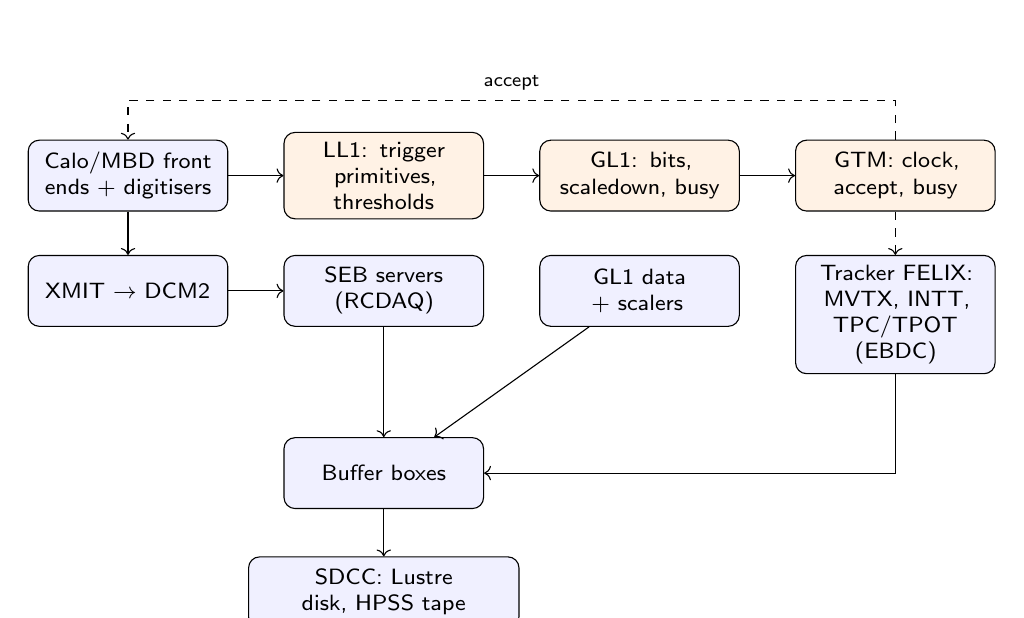
\begin{tikzpicture}[node distance=0.55cm and 0.7cm, box/.style={draw,rounded corners,fill=blue!6,align=center,font=\footnotesize,minimum height=0.9cm,text width=2.3cm}, tbox/.style={draw,rounded corners,fill=orange!10,align=center,font=\footnotesize,minimum height=0.9cm,text width=2.3cm}]
\node[box] (fe) {Calo/MBD front ends + digitisers};
\node[tbox,right=of fe] (ll1) {LL1: trigger primitives, thresholds};
\node[tbox,right=of ll1] (gl1) {GL1: bits, scaledown, busy};
\node[tbox,right=of gl1] (gtm) {GTM: clock, accept, busy};
\node[box,below=of fe] (dcm) {XMIT $\to$ DCM2};
\node[box,right=of dcm] (seb) {SEB servers (RCDAQ)};
\node[box,below=of gtm] (felix) {Tracker FELIX: MVTX, INTT, TPC/TPOT (EBDC)};
\node[box,below=of gl1] (gl1d) {GL1 data + scalers};
\node[box,below=1.4cm of seb] (bb) {Buffer boxes};
\node[box,below=0.6cm of bb,text width=3.2cm] (sdcc) {SDCC: Lustre disk, HPSS tape};
\draw[->] (fe) -- (ll1); \draw[->] (ll1) -- (gl1); \draw[->] (gl1) -- (gtm);
\draw[->] (fe) -- (dcm); \draw[->] (dcm) -- (seb);
\draw[->,dashed] (gtm.south) -- (felix.north);
\draw[->,dashed] (gtm.north) -- ++(0,0.5) -| node[pos=0.25,above,font=\scriptsize]{accept} (fe.north);
\draw[->] (seb) -- (bb); \draw[->] (felix.south) |- (bb.east); \draw[->] (gl1d) -- (bb);
\draw[->] (bb) -- (sdcc);
\end{tikzpicture}
\caption{Schematic trigger and data flow (simplified, after [S13]). Orange: trigger path; blue: data path. The GTM distributes the clock and accepts to all granules, including the tracker readout.}\label{fig:flow}
\end{figure}

\subsection{Trigger types}
The trigger menu includes [S13]:
\begin{itemize}
\item \textbf{Clock} (every crossing; heavily scaled down) and \textbf{random} triggers --- unbiased samples, used for noise, pedestals and zero-bias studies.
\item \textbf{MBD} north/south coincidences, with and without online vertex cuts --- the minimum-bias trigger.
\item \textbf{ZDC} north/south coincidences --- neutron-based; used e.g.\ for luminosity and UPC studies.
\item \textbf{Photon} triggers --- EMCal energy above thresholds (several thresholds, e.g.\ the ``Photon 3 GeV'' and ``Photon 4 GeV'' triggers you use).
\item \textbf{Jet} triggers --- EMCal+HCal energy in a larger window above thresholds.
\item \textbf{Cosmic} triggers, for calibration outside beam.
\item Pair and UPC triggers exist in the hardware design but have not been used [S13].
\end{itemize}
Each trigger is a \emph{bit} in a 64-bit word recorded by GL1 for every accepted crossing.
The bit assignments and trigger names are defined per run, and they \emph{changed within} Run 24 [S13].

\pitfallbox{Never hard-code a trigger bit number for a whole data set without checking the trigger names for each run. The bits you use (MB bit 10, Photon bits 29 and 30) are correct only for the run range where the menu had that layout. Use the per-run trigger names from the DAQ database or the \code{TriggerRunInfo} object (Section~\ref{sec:f4a}).}

%=====================================================================
\section{The MBD trigger and the online vertex}\label{sec:mbd}
\goal{Understand how the minimum-bias trigger is formed and what its vertex cut does.}

\subsection{MBD recap}
The MBD (Minimum Bias Detector, the former PHENIX beam--beam counters) consists of two arrays of quartz-radiator PMTs, north and south, at $z\approx\pm250$ cm, covering about $3.5<|\eta|<4.6$ [R1, S08].
Each PMT signal is split into a charge channel and a fast timing channel; the timing channel reaches a resolution of tens of picoseconds [S08].
The MBD samples every crossing and selects collisions with high efficiency; in Au+Au it can operate at collision rates of tens of kHz or more [S08].

\subsection{Time and vertex}
Let $t_N$ and $t_S$ be the arrival times of the fastest particles in the north and south arrays.
For a collision at position $z$ and time $t_0$ (with the arrays at $\pm L$):
\begin{equation}
t_N=t_0+\frac{L-z}{c},\qquad t_S=t_0+\frac{L+z}{c}\quad\Longrightarrow\quad z=\frac{c\,(t_S-t_N)}{2},\qquad t_0=\frac{t_N+t_S}{2}-\frac{L}{c}.
\end{equation}
Each arm's time is taken from a fit to the earliest cluster of PMT times above a charge threshold, to suppress late secondaries [S08].

\workedbox{timing needed for a vertex cut}{$z=10$ cm corresponds to $t_S-t_N=2z/c=0.67$ ns; $z=1$ cm to 67 ps. An online cut at $|z|<10$ cm therefore needs the arm-time difference to well below a nanosecond, which is why the timing channels are optimised for tens of ps. The offline MBD vertex is better than the online one because it uses full calibrations.}

\subsection{Minimum-bias trigger definitions}
A typical MB trigger requires at least $n$ hit PMTs in \emph{each} arm (a north--south coincidence), optionally with an online vertex window (for example $|z|<10$ cm, or a wide window of $|z|<150$ cm) [S13, S21].
The vertex-cut versions select collisions inside the silicon acceptance; the crossing angle of the beams is tuned so that many collisions occur within $|z|<10$ cm [S08].
The MB trigger is the normalisation trigger for most analyses: its \emph{visible cross section} $\sigma_{\rm MBD}$, measured with Vernier scans (Module 9) [S41], converts MB counts into luminosity.

\connectbox{Your analysis requires the MB trigger (bit 10 in your runs) for the minimum-bias sample and uses the MBD vertex.
Two consequences: (1) the MBD efficiency for events containing a high-$p_T$ $\pi^0$ is higher than for an average inelastic collision (hard events have more forward particles) --- this ``trigger bias'' must be in your normalisation; (2) the online vertex cut and the offline $|z_{\rm vtx}|$ cut differ in resolution, so near the cut boundary events migrate. Apply an offline cut somewhat inside the online window.}

%=====================================================================
\section{Calorimeter triggers}\label{sec:calotrig}
\goal{Understand how Photon and Jet triggers are formed, why their turn-on is not a step function, and how to measure their efficiency.}

\subsection{Trigger primitives and thresholds}
The LL1 receives digitised calorimeter data for every crossing, forms sums over groups of towers (trigger primitives), and combines neighbouring primitives into sliding windows [S13].
A Photon trigger fires when the maximum EMCal window sum exceeds a threshold; a Jet trigger uses larger windows of EMCal and HCal energy.
Several thresholds run in parallel (for example the Photon 3 and 4 GeV triggers you use, and Jet triggers at 6 and 8 GeV [S21]), each with its own scaledown.
The exact window sizes and threshold definitions are configuration; check the trigger documentation and the emulator (below) for your run period.

\subsection{Online versus offline energy}
The trigger uses an \emph{online} energy estimate: fast sums of ADC values, multiplied by online gains, in fixed geometric windows.
Your offline photon energy is a calibrated cluster energy from template-fitted towers (Module 3).
The two differ because of: (i) different calibrations; (ii) the window does not match the cluster shape (a cluster on a window boundary is split); (iii) noise and pedestal treatment; (iv) the underlying event and pile-up add to the window.
As a result the trigger efficiency as a function of offline energy is a smooth \textbf{turn-on curve}, not a step.

\subsection{Turn-on curves}
If the online estimate $E_{\rm on}$ is Gaussian-distributed around $kE_{\rm off}$ with width $\sigma(E)$, the probability to exceed a threshold $T$ is
\begin{equation}
\varepsilon(E_{\rm off})=\frac12\left[1+\mathrm{erf}\!\left(\frac{kE_{\rm off}-T}{\sqrt2\,\sigma}\right)\right].
\end{equation}
The 50\% point is at $E_{\rm off}=T/k$, and the width of the turn-on is $\sigma/k$.
Analyses usually use a trigger only above its \emph{plateau}, where $\varepsilon\approx1$, or correct for $\varepsilon(E)$ explicitly.

\workedbox{where is the plateau?}{Toy: $T=4$ GeV, $k=1$, $\sigma=0.6$ GeV. Then $\varepsilon(4)=50\%$, $\varepsilon(5)=95\%$, $\varepsilon(5.4)=99\%$, $\varepsilon(6)=99.9\%$. For a $\pi^0$ the trigger usually fires on the leading photon, which carries more than half of the $\pi^0$ energy, so the $\pi^0$ turn-on in $p_T$ is at lower $p_T$ than twice the photon threshold but is wider. (Toy numbers.)}

\subsection{Measuring the trigger efficiency}
The standard method uses an independent reference trigger (tag and probe):
\begin{equation}
\varepsilon_{\rm Photon}(E)=\frac{N(\text{MB-triggered},\ \text{Photon bit fired},\ E)}{N(\text{MB-triggered},\ E)}.
\end{equation}
The key is that GL1 records, for every accepted crossing, which triggers \emph{fired} (raw/live vectors), not only which trigger caused the readout (scaled vector). So in an MB-selected event you can check whether the Photon condition was satisfied, even if the Photon trigger was not the reason the event was recorded.
An alternative is a \textbf{trigger emulator}: apply the trigger algorithm in software to the recorded tower data. \code{TriggerAnalyzer} has an emulator option (\code{UseEmulator}) in the current software [R5].

\pitfallbox{\begin{itemize}
\item Using the scaled vector instead of the raw/live vector in the efficiency numerator: a Photon trigger with a scaledown would then look inefficient.
\item Measuring the turn-on in one run period and applying it to another with different online gains or thresholds.
\item Forgetting that hot towers can fire the trigger: a hot tower gives a trigger that fires without a real photon. Such towers are masked online and should be masked in the emulator.
\end{itemize}}

\connectbox{For your cross section the Photon-3 and Photon-4 triggers (bits 29 and 30 in your runs) supply the high-$p_T$ $\pi^0$ and $\eta$ samples. You need, for each, (1) the turn-on in $\pi^0$ $p_T$ measured from MB data (or emulated), (2) the $p_T$ above which you use the trigger, and (3) its effective luminosity (Section~\ref{sec:scalers}). Where two triggers overlap in $p_T$, compare their corrected spectra as a consistency check.}

\subsection{Out-of-time pile-up in the calorimeter readout window}
The calorimeter readout keeps a short train of samples per channel (16 samples of about 17.7 ns in recent runs [S15]), i.e.\ about 280 ns, or between two and three bunch crossings.
A collision in a neighbouring crossing produces a pulse shifted by $\pm106$ ns, i.e.\ by about six samples.
In the template fit such a pulse either distorts the fitted waveform (large $\chi^2$, flagged by \code{CaloTowerStatus}) or is fitted as a signal at the wrong time [S15].
With $\mu$ collisions per crossing on average, the probability that at least one of the two neighbouring crossings on each side contains a collision is $1-e^{-4\mu}$.

\workedbox{how often is there out-of-time energy? (toy)}{For $\mu=0.01$: $1-e^{-0.04}\approx4\%$ of triggered events have an extra collision within $\pm2$ crossings. For $\mu=0.04$: about 15\%. Most such collisions are soft and deposit little energy in any given tower, but the tail matters for isolation energy and for low-energy clusters. A cut on the calibrated cluster time, close to zero, removes most out-of-time energy at the cluster level. (Toy $\mu$ values.)}

\connectbox{Your cluster selection should include a timing requirement (calibrated tower or cluster time near zero) and a $\chi^2$/status requirement. Both reject out-of-time pile-up and distorted pulses. Their efficiency for real in-time photons must be measured (e.g.\ from the $\pi^0$ peak yield with and without the cut) and applied in the cross section.}

%=====================================================================
\section{Designing a trigger menu: bandwidth and scaledowns}\label{sec:menu}
\goal{Understand how scaledowns are chosen and why they change during a store.}
The DAQ can write a limited number of events per second, $B$. Each trigger $i$ has a live rate $R_i$. The scaledowns $s_i$ must satisfy
\begin{equation}
\sum_i\frac{R_i}{s_i+1}-(\text{overlaps})\ \le\ B,
\end{equation}
where ``overlaps'' accounts for events that satisfy several triggers but are written only once.
Rare triggers (high-threshold Photon and Jet) are given $s=0$ so that every live occurrence is recorded. Common triggers (MB, clock) receive large scaledowns, chosen to give each the bandwidth it needs.
The collision rate falls during a store as the beams burn off, so the scaledowns of the common triggers are lowered during the store to keep the total near $B$; this is one reason the scaledown can change within a run period and why $L^{\rm eff}$ must be summed segment by segment.

\workedbox{a toy menu}{Toy budget $B=10$ kHz. Live rates: MB 300 kHz, Photon-3 800 Hz, Photon-4 200 Hz, Jet-8 300 Hz, clock 9.4 MHz.
Give the rare triggers $s=0$: they use $800+200+300=1.3$ kHz (less after removing overlaps, since most Photon-4 events also fire Photon-3).
Allocate 3 kHz to MB: $s_{\rm MB}=300/3-1=99$.
Allocate 100 Hz to clock: $s_{\rm clock}\approx9.4\times10^6/100-1\approx94\,000$.
The rest of the budget goes to other triggers (lower thresholds, ZDC, calibration triggers).
Halfway through the store, with MB at 150 kHz, the same 3 kHz allocation needs $s_{\rm MB}=49$. (Toy rates.)}

%=====================================================================
\section{Scalers, scaledowns, live time and luminosity}\label{sec:scalers}
\goal{Be able to read GL1 scalers and turn them into an effective integrated luminosity for each trigger.}

\subsection{Raw, live and scaled}
For each trigger bit, GL1 keeps three running counters [S13]:
\begin{itemize}
\item \textbf{raw}: how many crossings satisfied the trigger condition (keeps up with the beam clock);
\item \textbf{live}: how many of those occurred while the DAQ was able to accept (not busy);
\item \textbf{scaled}: how many were actually accepted after the scaledown.
\end{itemize}
The \textbf{scaledown} $s$ is defined by $N_{\rm scaled}=N_{\rm live}/(s+1)$, i.e.\ $s=N_{\rm live}/N_{\rm scaled}-1$ [S13].
$s=0$ means every live trigger is taken; a disabled trigger is marked ``off''.
The \textbf{live fraction} is $N_{\rm live}/N_{\rm raw}$; it is the same for all bits to first order, because busy blocks everything.
A per-event record of the same information is kept: in each accepted event GL1 stores the \emph{trigger} (raw) vector, the \emph{live} vector and the \emph{scaled} vector as 64-bit words, plus the bunch number [R5].

\subsection{Dead time and multi-event buffering}
After each accept the front ends need time to digitise and ship the data.
If the system could hold only one event at a time, the dead time per event $\tau$ would give a live fraction $1/(1+R\tau)$ for an accept rate $R$ (non-paralysable dead time).
sPHENIX uses \textbf{multi-event buffering} (MEB): the front ends can hold several accepted events at once, so a second good trigger right after the first is not lost; only a short, unavoidable dead time after each accept remains [S13].
When all buffers are full, the system is busy until one is freed.

\workedbox{live time (toy)}{With a single buffer and $\tau=10\ \mu$s, an accept rate of 10 kHz gives a live fraction $1/(1+0.1)=91\%$; 15 kHz gives 87\%. If $\tau=30\ \mu$s, 15 kHz gives 69\%. Multi-event buffering moves the busy condition from ``one event in flight'' to ``all buffers in flight'', which raises the live fraction at a given rate. (Toy parameters.)}

\subsection{From scalers to luminosity}
The integrated luminosity seen by a trigger is the number of collisions it could have recorded divided by the cross section:
\begin{equation}
L_{\rm MB}=\frac{N^{\rm MB}_{\rm live}}{\sigma_{\rm MBD}}\quad(\text{luminosity while live}),\qquad L^{\rm eff}_{X}=\frac{N^{\rm MB}_{\rm live}}{(s_X+1)\,\sigma_{\rm MBD}}\quad(\text{effective, for trigger }X).
\end{equation}
Here $\sigma_{\rm MBD}$ is the visible MB cross section (from a Vernier scan, Module 9) and $s_X$ the scaledown of trigger $X$.
For a Photon trigger with $s=0$, $L^{\rm eff}$ equals the live MB luminosity of the same period (if the Photon trigger and the MB trigger share the same live time).
If $s$ changes during a run (it can), sum the contributions period by period.

\subsection{Pile-up correction to MB counts}
The MB scaler counts \emph{crossings with at least one} MBD coincidence, not collisions.
With Poisson statistics and $\mu$ collisions per crossing on average, the fraction of crossings with at least one collision is $p=1-e^{-\mu}$, so
\begin{equation}
\mu=-\ln\!\left(1-\frac{N_{\rm MB}}{N_{\rm crossings}}\right),\qquad N_{\rm coll}=\mu\,N_{\rm crossings}\ \ge\ N_{\rm MB}.
\end{equation}
The number of crossings comes from the beam-clock scaler (restricted to filled bunches).
The correction $N_{\rm coll}/N_{\rm MB}=\mu/(1-e^{-\mu})\approx1+\mu/2$ is small at low rate but not negligible at high rate [S16].

\subsection{Trigger bias of the minimum-bias condition for hard events}
The MB trigger does not fire for every inelastic collision. Its visible cross section is $\sigma_{\rm MBD}=\varepsilon^{\rm inel}_{\rm MBD}\,\sigma_{\rm inel}$.
Events containing a hard scattering (e.g.\ a high-$p_T$ $\pi^0$) produce more forward particles on average, so the MBD fires for them with a \emph{different} (usually higher) efficiency $\varepsilon^{\pi^0}_{\rm MBD}$.
For a yield $N_{\pi^0}$ measured in MB-triggered events,
\begin{equation}
\sigma_{\pi^0}=\frac{N_{\pi^0}}{\varepsilon^{\pi^0}_{\rm MBD}\,L},\qquad L=\frac{N_{\rm MB}}{\sigma_{\rm MBD}}\quad\Longrightarrow\quad\sigma_{\pi^0}=\frac{N_{\pi^0}}{N_{\rm MB}}\,\frac{\sigma_{\rm MBD}}{\varepsilon^{\pi^0}_{\rm MBD}}.
\end{equation}
The ratio $\varepsilon^{\pi^0}_{\rm MBD}$ must be estimated, for example from simulation (PYTHIA8 events through the MBD simulation, comparing events with and without a high-$p_T$ $\pi^0$), or in data from a sample triggered without the MBD (e.g.\ a calorimeter trigger without MBD requirement, if one is in the menu, or clock/random triggers if statistics allow).
The same reasoning applies to the online/offline vertex cut: if the $\pi^0$ yield and the MB count use the same vertex window, the vertex acceptance largely cancels, but the vertex-finding efficiency may differ between hard and average events.

\workedbox{luminosity for your normalisation (toy)}{Suppose the MB live counter for a run period reads $N^{\rm MB}_{\rm live}=4.0\times10^{9}$ and $\sigma_{\rm MBD}=25$ mb (toy). Then $L_{\rm MB}=4.0\times10^9/25\ \mathrm{mb}=1.6\times10^8\ \mathrm{mb^{-1}}=0.16\ \mathrm{pb^{-1}}$.
If the MB trigger itself had $s=99$, the recorded MB sample corresponds to $0.0016\ \mathrm{pb^{-1}}$; a Photon trigger with $s=0$ in the same period corresponds to the full 0.16 pb$^{-1}$.
If $\mu=0.04$, the pile-up correction is $\approx1.02$, i.e.\ a 2\% effect on $L$. (Toy numbers; real values come from the scalers and the Vernier-scan analysis.)}

\connectbox{Your invariant cross section is
$E\,\mathrm{d}^3\sigma/\mathrm{d}p^3=\frac{1}{2\pi p_T}\frac{N_{\pi^0}(p_T)}{L^{\rm eff}\,\varepsilon\,\mathrm{BR}\,\Delta p_T\Delta y}$.
The GL1 scalers enter through $L^{\rm eff}$: live MB counts per segment of constant scaledown, divided by $(s+1)$ for the MB sample and by $\sigma_{\rm MBD}$. Check (1) that you use \emph{live} not raw counts; (2) that segments with different scaledowns are summed separately; (3) the pile-up correction; (4) that the MBD vertex efficiency and the offline $|z|$ cut are treated consistently between $N_{\pi^0}$ and $L$.}

%=====================================================================
\section{The DAQ: from front ends to storage}\label{sec:daq}
\goal{Know where the data go after an accept, and what the raw files look like.}

\subsection{Data paths}
\begin{itemize}
\item \textbf{Calorimeters, MBD, sEPD, ZDC:} digitiser crates send data through transmitter modules (XMIT) to DCM2 boards, which package the data and report busy; the packaged data go to sub-event buffer servers (SEBs) [S13].
\item \textbf{TPC and TPOT:} FELIX boards in event-buffering and data-collector servers (EBDCs) [S13].
\item \textbf{MVTX and INTT:} their own FELIX servers [S13].
\item \textbf{GL1:} its own data stream with the trigger words and scalers.
\end{itemize}
Every readout server runs \textbf{RCDAQ}, the DAQ software, which collects the packaged data for that granule and writes it out. Data are not stored on these machines; they are transferred to the \textbf{buffer boxes} [S13].
RCDAQ supports triggered, extended and streaming formats in one framework [S13].

\subsection{Buffer boxes and storage}
The buffer boxes are large disk servers in the counting house (of order a petabyte each). Their only job is to receive data from the readout servers and transfer them to SDCC, where the raw files are archived to tape (HPSS) and staged to disk (Lustre) for production [S13].
If transfer stopped, the buffer boxes would fill within weeks [S13].
The calorimeter systems alone write data at the GB/s scale during physics running; the trackers write much more [S13].

\subsection{Raw data format}
Raw files use the PRDF format (PHENIX raw data format). A file contains events; an event contains \emph{packets}; each packet holds the data of one readout unit, with headers identifying it [S13].
For a calorimeter packet the words include a transmitter header, an ADC-board header, the channel data (zero-suppressed channels with two samples, unsuppressed channels with the full waveform), and checksum words [S13].
The unpacking into waveforms is done offline by the decoders in \code{fun4allraw}/\code{ffarawobjects} and then by \code{CaloTowerBuilder} (Module 3).

\workedbox{why zero suppression matters}{One EMCal event with full waveforms in every channel would be $24\,576\ \mathrm{channels}\times16\ \mathrm{samples}\times2\ \mathrm{bytes}\approx0.79$ MB. With zero suppression, most channels keep only two samples: $24\,576\times2\times2\approx0.10$ MB, plus full waveforms for the few channels with signal. At several kHz of accepts this is the difference between a few GB/s and several hundred MB/s for one subsystem. (Approximate; header overheads ignored.)}

\subsection{Event combining}
Raw data are written as one file stream per readout server.
To build a physics event, offline \textbf{event combining} aligns the sub-events from all servers belonging to the same crossing, using event counters and beam-clock (BCO) values, so that event $n$ in the output contains data from the same collision in every subsystem [S13, S15].
Desynchronisation (one server shifted by one event) is a classic failure mode; it shows up as lost correlations between subsystems (e.g.\ EMCal energy vs.\ MBD charge, INTT clusters vs.\ MBD charge [S11]).

\checksbox{\begin{itemize}
\item Correlation of total EMCal energy with MBD charge sum, event by event: a cloud along a diagonal means synchronised data; an uncorrelated blob means misaligned events.
\item GL1 bunch numbers in the event must be consistent with the filled-bunch pattern.
\item Scaled counts per run should equal the number of events in the run's DSTs with the corresponding scaled bit set (up to events lost in production).
\end{itemize}}

%=====================================================================
\section{Triggered, extended and streaming readout}\label{sec:stream}
\goal{Understand the three readout modes, which detectors use which, and how to analyse streaming data.}

\subsection{The three modes}
\begin{itemize}
\item \textbf{Triggered:} a detector records data only for the accepted crossing (calorimeters: a few samples around it).
\item \textbf{Extended readout:} on a trigger, a detector records a long window (MVTX: one long strobe; INTT: of order a hundred crossings; TPC: a frame of tens of $\mu$s instead of just the 13 $\mu$s drift), so that out-of-time collisions around the trigger are also recorded [S10, S11, S21].
\item \textbf{Streaming:} a detector records continuously, independent of the trigger. The MVTX issues back-to-back strobes of about 10 $\mu$s; the INTT sends every hit with its crossing number; the TPC sends consecutive frames prompted by a clock trigger [S10, S11, S21].
\end{itemize}

\subsection{Who streams?}
The tracking detectors (MVTX, INTT, TPC; TPOT has the capability but does not use it) can stream. The calorimeters, sEPD, MBD and ZDC are triggered only [S21].
Corollary: a streaming analysis is a \emph{tracking} analysis; there is no guarantee of calorimeter data for an arbitrary crossing [S21].
The configuration changed between data-taking periods. Broadly: in Run-24 $p$+$p$ the MVTX streamed, the INTT was triggered at first and later streamed, and the TPC used extended readout; in Run-25 Au+Au all trackers were triggered (the MVTX because of beam-background conditions); in Run-25 $p$+$p$ and O+O the trackers streamed, the TPC with a configurable streaming fraction that was limited by data rate early in each store [S21].

\subsection{Why stream?}
Some physics cannot be triggered efficiently with calorimeters: low-$p_T$ heavy-flavour hadronic decays ($D^0$, $B$), $\Upsilon$ reconstruction from tracks, low-$p_T$ light-flavour hadrons for spin asymmetries [S21].
These need a very large \emph{zero-bias} sample reconstructed offline.
Streaming provides exactly that: every crossing in the streaming windows, with an effective luminosity much closer to the delivered luminosity than any prescaled MB trigger [S21].

\workedbox{streaming versus a prescaled trigger}{In one hour RHIC provides $9.38\times10^6\ \mathrm{s^{-1}}\times3600\ \mathrm{s}\approx3.4\times10^{10}$ crossings. A fully streamed tracking readout records all of them. A clock trigger with a scaledown of order $10^5$ records only a few hundred thousand of them. For a ``common'' trigger that is heavily scaled down, the streaming sample contains far more collisions than the triggered sample; for a ``rare'' trigger with $s=0$, the two are similar (streaming has no trigger dead time, so it is slightly larger) [S21]. (Derived from the crossing rate; scaledown illustrative.)}

\subsection{Luminosity plots: sampled vs recorded}
Run-summary plots show a ``triggered'' luminosity larger than the ``streaming'' one. This is not a contradiction: the triggered number is the luminosity \emph{sampled} by the trigger (before scaledown), while the streaming number is \emph{recorded}. Moreover, the TPC streaming fraction is below 100\% and lowest at the start of a store, exactly when the collision rate is highest [S21].
Counting the streaming luminosity is non-trivial; a first implementation is the \code{StreamingLumiReco} module in the coresoftware \code{bcolumicount} package [S21, R5].

\subsection{Analysing streaming data}
\begin{enumerate}
\item \textbf{Readout frames.} Offline, the event combiner builds frames of about 50 $\mu$s (set by the TPC frame) around each GL1 trigger: it finds the MVTX strobes and INTT hits that fall in the TPC window and groups them into one Fun4All ``event'' [S21].
\item \textbf{Track finding constraints.} MVTX clusters on a track must share a strobe; INTT clusters must have the same crossing number within $\pm1$; TPC seeds are matched spatially to silicon seeds; a track's crossing is the crossing of its INTT clusters [S21].
\item \textbf{Crossings, not events.} A collision is identified by (event number, crossing number). Crossing 0 is the triggered crossing. A 50 $\mu$s frame spans about 470 crossings, but only those whose TPC drift is fully contained are complete; in practice about crossings 1--360 are usable, and those below 0 or above that range see a partial drift [S21].
\item \textbf{Exclude the triggered crossing.} It is biased by the trigger. All other crossings should be statistically equivalent; correcting the bias would recover only about 10\% more statistics [S21].
\item \textbf{Remove duplicates.} Consecutive frames can overlap if triggers are closer than one frame length; then the same tracks appear twice. Check whether the GL1 BCO difference between frames is smaller than the frame size; if so, drop tracks in the later frame whose parameters match a track in the earlier frame with a crossing shift equal to the BCO difference [S21].
\item \textbf{QA vs crossing.} Any observable (e.g.\ the $K^0_S$ peak position, width and yield) should be flat versus crossing number, except at crossing 0. Deviations indicate crossing mis-assignment, partial drift or duplication [S21].
\item \textbf{Simulate streaming conditions.} Simulations must reproduce the streaming readout (pile-up in the frame, crossing assignment) for closure tests [S21].
\end{enumerate}

\begin{figure}[!htbp]\centering
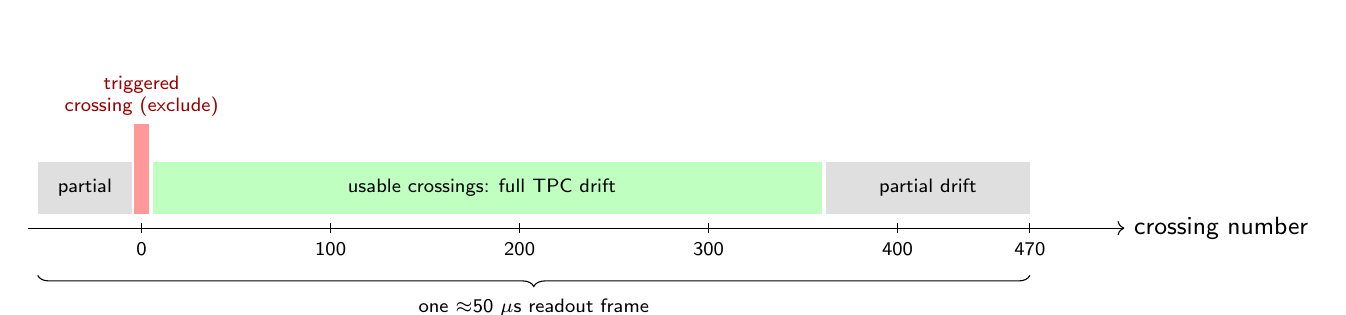
\begin{tikzpicture}[xscale=0.024,yscale=0.6]
\draw[->] (-60,0) -- (520,0) node[right,font=\small] {crossing number};
\foreach \x in {0,100,200,300,400,470} \draw (\x,0.1) -- (\x,-0.1) node[below,font=\scriptsize] {\x};
\fill[red!40] (-4,0.3) rectangle (4,2.2); \node[red!60!black,font=\scriptsize,align=center] at (0,2.8) {triggered\\crossing (exclude)};
\fill[green!25] (6,0.3) rectangle (360,1.4); \node[font=\scriptsize] at (180,0.85) {usable crossings: full TPC drift};
\fill[gray!25] (-55,0.3) rectangle (-5,1.4); \node[font=\scriptsize,align=center] at (-30,0.85) {partial};
\fill[gray!25] (362,0.3) rectangle (470,1.4); \node[font=\scriptsize] at (416,0.85) {partial drift};
\draw[decorate,decoration={brace,mirror,amplitude=4pt}] (-55,-1.0) -- (470,-1.0) node[midway,below=5pt,font=\scriptsize] {one $\approx$50 $\mu$s readout frame};
\end{tikzpicture}
\caption{Schematic of a streaming readout frame (approximate ranges, after [S21]). Not to scale in detail.}\label{fig:frame}
\end{figure}

\subsection{Getting tracks out}
Track DSTs (\code{DST\_TRACK\_*}, together with \code{DST\_CLUSTER\_*} and \code{DST\_SEED\_*}) contain \code{SvtxTrackMap} and \code{SvtxVertexMap} [S21].
Ready-made modules write TTrees: \code{TrackResiduals} (reconstructed tracks, states and residuals; the main tool for data), \code{SvtxEvaluator} (simulation, with truth matching; slow), and \code{KFParticle\_sPHENIX} (secondary vertices and decays, used in light- and heavy-flavour analyses) [S21].
A ready macro is \code{macros/TrackingProduction/Fun4All\_TrackAnalyzer.C} [S21].

\connectbox{Your $\pi^0$/$\eta$ analysis is calorimeter-based and therefore uses \emph{triggered} data only. Streaming matters to you in two ways: (1) any track-based cross-check (charged-track veto, conversion tagging, track vertex) must use the triggered crossing (crossing 0) of each event, because the calorimeter data exist only for that crossing; (2) when you read a luminosity plot, distinguish triggered (sampled) from streaming (recorded) luminosity.}

%=====================================================================
\section{From raw data to DSTs, and finding files}\label{sec:prod}
\goal{Know the production chain, the DST types, the tag scheme, and how to list files.}

\subsection{The production chain}
\begin{enumerate}
\item \textbf{Raw PRDF files} (one stream per readout server) arrive on SDCC storage.
\item \textbf{Event combining} builds aligned events (triggered) or frames (streaming) [S13, S21].
\item \textbf{First-pass reconstruction} writes DSTs. For the calorimeters, \code{CaloTowerBuilder} fits the waveforms and writes uncalibrated \code{TowerInfo} towers; this is the \code{DST\_CALOFITTING} stage, and it is essentially all that is stored from the calorimeters at that point [S13, S15].
\item \textbf{Later passes} apply calibrations and produce higher-level DSTs (calibrated calorimeter objects, clusters; tracking clusters, seeds and tracks; global objects).
\item \textbf{QA} histograms are produced alongside (\code{HIST\_*} types), and runs are classified good or bad (Module 9).
\end{enumerate}
Productions are run centrally on SDCC by the production team; you read their output.

\subsection{Tags and file names}
A production is identified by a \textbf{tag} of the form \code{<build>\_<cdb>\_<version>}: the software build (e.g.\ an \code{ana.NNN} release), the conditions-database global tag used (e.g.\ \code{2024pNNN}), and a version number when the same build/CDB combination was produced more than once [R5].
DST file names combine the DST type, the dataset (run period and species, e.g.\ \code{run2pp} for the 2024 $p$+$p$ run), the tag, the run number (zero-padded) and the segment number:
\begin{verbatim}
DST_<TYPE>_<dataset>_<build>_<cdb>[_<version>]-<run>-<segment>.root
\end{verbatim}
A run is split into many segments (files) of similar size. A complete run analysis must include all segments.

\subsection{The FileCatalog and \code{CreateDstList.pl}}
Metadata for all production files (dataset, type, tag, run, segment, location on Lustre or HPSS) live in the FileCatalog database. The command-line tool \code{CreateDstList.pl} queries it and writes file lists for Fun4All input managers. Its options in the current release include [R5]:
\begin{verbatim}
CreateDstList.pl --printtags --dataset run2pp          # which tags exist
CreateDstList.pl --printdsttypes --dataset run2pp --tag <tag>
CreateDstList.pl --printruns --dataset run2pp --tag <tag>
CreateDstList.pl --tag <tag> --run <run> <dsttype>     # list of segments
CreateDstList.pl --tag <tag> --list runs.txt <dsttype> # many runs
\end{verbatim}
(\code{--tag} is mandatory for file lists; \code{--hpss} lists files on tape; check the usage message of your release.) \code{CreateFileList.pl} plays the same role for simulation productions.

\pitfallbox{\begin{itemize}
\item Mixing tags: two tags of the same run differ in calibration. Use one tag for the whole data set, or treat the difference as a systematic.
\item Missing segments: a run with segments that failed in production has fewer events than the scalers suggest. Your luminosity must be computed for the events you actually analysed (e.g.\ from GL1 scaler differences between the first and last event of each segment, or by counting MB events).
\item Assuming the DST type name is the same in every production: check \code{--printdsttypes}.
\end{itemize}}

%=====================================================================
\section{Run information: the DAQ database and monitoring}\label{sec:db}
\goal{Know where to find what happened during a run.}
\begin{itemize}
\item \textbf{Run pages} on the internal web summarise each run (duration, triggers, subsystems, event counts). They are easy to use but limited in search [S13].
\item \textbf{The DAQ database} (PostgreSQL; a read-only replica is reachable from SDCC interactive nodes with \code{psql}) holds the full record. With some SQL you can: get basic run information; list which triggers were active and their names and scaledowns for a run; filter runs by triggers enabled or disabled; and see which subsystems (readout granules) were included in a run [S13]. Learning basic SQL is a transferable skill.
\item \textbf{Grafana} dashboards show time histories (rates, voltages, temperatures, data rates) for any time window [S13].
\end{itemize}
Most of what you take from these sources is a \emph{run veto}: runs without a required subsystem, with the wrong trigger configuration, too short, or with known problems are removed. Within good runs, you then select events by trigger bits [S13].

%=====================================================================
\section{Trigger information inside a Fun4All module}\label{sec:f4a}
\goal{Read trigger bits and scalers in your own code.}

\subsection{Directly from \code{Gl1Packet}}
The GL1 data for each event are stored in a \code{Gl1Packet} object (\code{offline/framework/ffarawobjects}) on the node tree. Its accessors include [R5]:
\begin{itemize}
\item \code{getTriggerVector()}, \code{getLiveVector()}, \code{getScaledVector()}: 64-bit words, one bit per trigger;
\item \code{getBunchNumber()}: the crossing number in the RHIC fill pattern;
\item \code{getScaler(bit, index)}: the running raw/live/scaled counters for a bit (three counters per bit; check the index order in the source).
\end{itemize}
To test bit $b$: \code{(getScaledVector() >> b) \& 1}. You must know which bit is which trigger for that run [S13].

\subsection{With \code{TriggerAnalyzer} and \code{TriggerRunInfo}}
The \code{calotrigger} package provides helpers [R5]:
\begin{itemize}
\item \code{TriggerRunInfo} (filled by the \code{TriggerRunInfoReco} module) stores the per-run trigger names, scaledowns and scalers; e.g.\ \code{getTriggerName(bit)}, \code{getPrescaleByName(name)}, \code{getScalersByName(name)}.
\item \code{TriggerAnalyzer}: call \code{decodeTriggers(topNode)} once per event, then \code{didTriggerFire(name or bit)} (scaled), \code{checkRawTrigger(name or bit)} (raw), \code{getTriggerPrescale(...)}, and the scaler accessors \code{getTriggerScalers}, \code{getTriggerLiveScalers}, \code{getTriggerRawScalers}. Using names instead of bit numbers protects you from menu changes.
\end{itemize}
A sketch (suggested; check the current headers):
{\footnotesize\begin{verbatim}
// in process_event(PHCompositeNode *topNode)
m_trig->decodeTriggers(topNode);                // TriggerAnalyzer *m_trig
bool mb      = m_trig->didTriggerFire(10);        // or by name for your run range
bool photon4 = m_trig->checkRawTrigger(30);  // bit 30 in your runs;
                                              // verify: m_trig->getTriggerName(30)
// trigger efficiency numerator/denominator in MB-selected events:
if (mb) { h_den->Fill(Eclus); if (photon4) h_num->Fill(Eclus); }
\end{verbatim}}
(Bit numbers are valid only for the run range where the menu had this layout. Print the name of each bit for each run, or switch to the name-based calls once you have the exact names.)

%=====================================================================
\section{Computing access: ssh and web}\label{sec:ssh}
\goal{Set up secure, convenient access to SDCC and internal web pages.}

\subsection{Accounts, keys and the agent}
Access requires an SDCC (formerly RACF) account [S13].
Your account password is for administrative tasks; day-to-day logins should use \textbf{ssh keys}, which are far more secure: the server sends a random challenge encrypted with your public key, and only your secret key can answer it, so no reusable secret ever crosses the network [S13].
The SDCC gateways do not accept passwords at all [S13].
Recommended practice [S13]:
\begin{itemize}
\item Generate a strong key (\code{ssh-keygen -t rsa -b 4096 -f <name>}, or a modern ed25519 key), protected by a passphrase; use separate keys for separate roles (SDCC, GitHub, other labs).
\item Upload the public key through the SDCC account web page. Also place it in the file \code{authorized\_keys} in the \code{.ssh} directory of your SDCC home area (file mode 600, directory mode 700), transferring it via the SFTP gateway.
\item Unlock keys once per session with \code{ssh-add}; the \textbf{ssh-agent} holds them, and agent forwarding lets onward hops authenticate without typing anything.
\end{itemize}

\subsection{An \code{\textasciitilde/.ssh/config} that hides the gateways}
SDCC has two kinds of gateways: one in front of the SDCC computing nodes and one (``campus'') in front of machines on the BNL campus network; there is no direct path between the two zones [S13].
With \code{ProxyJump} rules your client hops through the right gateway automatically. A minimal version, with \code{<user>} replaced by your SDCC user name (after [S13]):
{\footnotesize\begin{verbatim}
ForwardAgent yes
ForwardX11 yes
Host ssh*.sdcc.bnl.gov cssh*.sdcc.bnl.gov
  User <user>
  ProxyCommand none
Host sphnx* rcas20*
  HostName %h.rcf.bnl.gov
  ProxyJump <user>@ssh.sdcc.bnl.gov
# keep this catch-all rule last
Host *.bnl.gov
  ProxyJump <user>@cssh.sdcc.bnl.gov
\end{verbatim}}
Then \code{ssh sphnx01} reaches an interactive node in one command. On Windows, an OpenSSH implementation (Cygwin, or the native Windows OpenSSH) accepts the same configuration; PuTTY needs its own translation of every setting [S13].
Only forward the agent to hosts you trust.

\subsection{Internal web pages without a VPN}
Internal pages (logbooks, run pages, wikis) are reachable through an ssh tunnel to a web proxy inside BNL, combined with a browser proxy manager that sends only URLs containing \code{bnl.gov} through the tunnel [S13].
Compared with a VPN this keeps your other traffic (home printer, personal browsing) off the BNL network and avoids accidental computer-use-agreement violations [S13].
The proxy host and port, and a ready configuration file, are given in the collaboration's internal tutorial.

%=====================================================================
\section{Good analysis code}\label{sec:code}
The streaming talk ended with advice that applies to every analysis [S21]: separate the reusable core from the specific case (e.g.\ a generic ``particle A / particle B'' ratio class); keep all configuration (binning, cuts, ranges) in one visible place; split large functions into steps; name things for what they do; reuse existing collaboration tools rather than standalone look-alikes; avoid copy-paste (if a block appears four times, write a loop); design the interface early if others will use it, and do not change it without warning; comment the \emph{why}; delete obsolete commented-out code. Code generated with AI assistants must be read, understood and cleaned to the same standard before it is pushed [S21].

\subsection*{A crossing's journey, end to end}
\begin{enumerate}
\item A $p$+$p$ collision produces a $\pi^0$ whose photons deposit 5 GeV in the EMCal; the MBD arms see forward particles.
\item The digitisers sample every channel continuously; LL1 sees an EMCal window sum above the Photon-4 threshold and the MBD sees a north--south coincidence.
\item GL1 sets the raw bits for Photon-4, Photon-3 and MB; the DAQ is live, so the live bits are set; Photon-4 has $s=0$, so the scaled bit is set and an accept is issued through the GTM.
\item The calorimeter front ends ship 16 samples per channel (two for zero-suppressed channels) via XMIT and DCM2 to the SEBs; the trackers deliver their extended or streaming data via FELIX; GL1 writes the trigger words and scalers.
\item RCDAQ on each server writes PRDF files to the buffer boxes, which transfer them to SDCC tape and disk.
\item Production combines the sub-events, fits the waveforms (\code{CaloTowerBuilder}) and writes \code{DST\_CALOFITTING} segments with a production tag; the FileCatalog records them.
\item You list the segments with \code{CreateDstList.pl}, run \code{CaloTowerStatus}/\code{CaloTowerCalib} and clustering, select events with \code{TriggerAnalyzer}, and normalise with the GL1 live MB scalers and $\sigma_{\rm MBD}$.
\end{enumerate}

%=====================================================================
\section{Summary}
\begin{itemize}
\item RHIC crosses at $\approx9.4$ MHz; the DAQ accepts of order 10 kHz; triggers select crossings.
\item LL1 forms calorimeter trigger primitives, GL1 forms the trigger bits and applies scaledowns and busy, GTM distributes clock and accepts.
\item MBD: north--south coincidence, timing vertex $z=c(t_S-t_N)/2$, vertex-selected MB triggers; MB is the luminosity reference.
\item Photon/Jet triggers use online sums; the offline turn-on is smooth; measure it with MB events using the raw/live trigger vector.
\item Scalers: raw, live, scaled; $s=N_{\rm live}/N_{\rm scaled}-1$; $L^{\rm eff}_X=N^{\rm MB}_{\rm live}/[(s_X+1)\sigma_{\rm MBD}]$, with a pile-up correction.
\item Data flow: XMIT/DCM2/SEB (calorimeters), FELIX/EBDC (trackers), RCDAQ, buffer boxes, SDCC tape and disk; PRDF packets; event combining.
\item Trackers can stream; calorimeters cannot. Streaming analysis works in crossings, excludes crossing 0, removes duplicates and checks stability vs crossing.
\item DSTs are identified by type, dataset, tag (build\_cdb\_version), run and segment; \code{CreateDstList.pl} lists them.
\end{itemize}

%=====================================================================
\section{Hands-on exercises on SDCC (optional, suggested)}
These exercises are optional. They have not been run as part of writing this module; commands are suggestions to be checked against the current release. The text does not depend on them.
\begin{enumerate}
\item \textbf{List the DST segments of one run (checkpoint).} Set up the environment and list the available tags:
\begin{verbatim}
source /opt/sphenix/core/bin/sphenix_setup.sh -n new
CreateDstList.pl --printtags --dataset run2pp
\end{verbatim}
Pick the tag used in your analysis, list the DST types with \code{--printdsttypes}, and write the list of \code{DST\_CALOFITTING} segments for one of your runs with \code{--run}. Count the segments and compare with the run page.
\item \textbf{Read the GL1 scalers for that run (checkpoint).} In a small \code{SubsysReco}, fetch the \code{Gl1Packet} in the first and the last event of the run (or of each segment) and print \code{getScaler(bit, i)} for $i=0,1,2$ for the MB bit and the two Photon bits. Compute live fraction, scaledown and the live MB count difference. Alternatively print the per-run values from \code{TriggerRunInfo}.
\item \textbf{Luminosity bookkeeping.} With a toy $\sigma_{\rm MBD}$, convert the live MB count from exercise 2 into pb$^{-1}$, then into the effective luminosity of each trigger. Add the pile-up correction using the crossing count.
\item \textbf{Turn-on curve.} In MB-triggered events of a few segments, fill the leading-cluster energy for all events and for events where the Photon-4 \emph{raw} bit fired; divide, and fit with the erf form. Repeat with the scaled bit to see the pitfall.
\item \textbf{Trigger menu changes.} Query the DAQ database (read-only replica, \code{psql}) for the trigger names of bits 10, 29 and 30 in your first and last Run-24 runs. Did they change?
\item \textbf{ssh config.} Write the \code{\textasciitilde/.ssh/config} of Section~\ref{sec:ssh} on your laptop and log into an interactive node in one command with your agent holding the key.
\end{enumerate}

%=====================================================================
\section{Self-test questions}
\begin{enumerate}
\item Why can sPHENIX not read out every crossing? Give the crossing rate and the order of magnitude of the accepted rate.
\item What are LL1, GL1 and GTM responsible for?
\item Derive the MBD vertex formula. What arm-time difference corresponds to $z=10$ cm?
\item Define raw, live and scaled counts. If the live count is 3000 and the scaled count is 1000, what is the scaledown?
\item A trigger has $s=0$ in one half of a run and $s=4$ in the other half; the live MB counts in the two halves are equal. What is its effective luminosity relative to the live MB luminosity?
\item Why is the Photon trigger efficiency, as a function of offline cluster energy, not a step function?
\item In measuring the Photon trigger efficiency with MB events, why must you use the raw (or live) trigger vector and not the scaled one?
\item What does multi-event buffering achieve?
\item What is the pile-up correction to MB counts, and when is it important?
\item Which sPHENIX detectors can stream? What follows for a calorimeter analysis?
\item In a streaming analysis, why is crossing 0 excluded, and how are duplicates created and removed?
\item What does the tag \code{<build>\_<cdb>\_<version>} encode, and why must one data set use a single tag?
\item What happens in event combining, and how would you detect a desynchronised subsystem?
\item Why are ssh keys with an agent more secure than passwords?
\item Why should a trigger bit number not be hard-coded for all of Run 24?
\end{enumerate}

\appendix
\section{Answers}
\begin{enumerate}
\item The beam clock gives $\approx9.4$ million crossings per second; full readout of everything would be of order PB/s. The DAQ accepts of order 10 kHz (about $10^{-4}$ s per event), so a selection of about one crossing in a thousand is needed.
\item LL1 computes trigger primitives and threshold decisions from digitised calorimeter (and MBD) data for every crossing. GL1 combines inputs into trigger bits, applies scaledowns and the busy veto and issues accepts. GTM distributes the beam clock and accepts to all readout granules and collects their busy signals.
\item $t_N=t_0+(L-z)/c$, $t_S=t_0+(L+z)/c$; subtracting gives $z=c(t_S-t_N)/2$. For $z=10$ cm, $t_S-t_N=0.67$ ns.
\item Raw: crossings satisfying the condition; live: those occurring while the DAQ could accept; scaled: those accepted after scaledown. $s=3000/1000-1=2$.
\item $L^{\rm eff}=\tfrac12L_{\rm live}/1+\tfrac12L_{\rm live}/5=0.6\,L_{\rm live}$.
\item The trigger uses online sums with online gains in fixed windows, which differ from the calibrated, clustered offline energy; the ratio fluctuates event by event (noise, window splitting, calibration differences), so the threshold is smeared into an erf-like turn-on.
\item The scaled vector says which triggers caused the readout after scaledown; a scaled-down Photon trigger would be missing in many events where its condition was satisfied, biasing the efficiency low. The raw/live vectors record whether the condition was satisfied.
\item It lets the front ends hold several accepted events at once, so closely spaced triggers are not lost; only a short fixed dead time per accept remains, raising the live fraction.
\item MB scalers count crossings with at least one collision; the number of collisions is $\mu N_{\rm crossings}$ with $\mu=-\ln(1-N_{\rm MB}/N_{\rm crossings})$, i.e.\ larger by $\approx1+\mu/2$. It matters at high collision rates (large $\mu$).
\item MVTX, INTT, TPC (and TPOT in principle). The calorimeters, MBD, sEPD and ZDC are triggered only, so calorimeter information exists only for triggered crossings; a calorimeter analysis uses triggered data, and any track information must come from the triggered crossing.
\item Crossing 0 is biased by the trigger condition. Duplicates arise when consecutive readout frames overlap in time (triggers closer than the frame length); they are removed by comparing the GL1 BCO difference with the frame size and discarding tracks in the later frame that match earlier ones shifted by that difference.
\item The software build, the conditions-database global tag (calibrations), and the production version. Different tags mean different calibrations or software, so mixing them introduces inconsistencies.
\item The sub-event streams from all readout servers are aligned so each output event contains data from the same crossing everywhere. A desynchronised subsystem destroys event-by-event correlations (e.g.\ EMCal energy vs MBD charge).
\item No reusable secret is transmitted: authentication answers a fresh random challenge with the secret key, which never leaves your machine; the agent avoids retyping the passphrase so it cannot be shoulder-surfed.
\item Trigger names and bit assignments changed within Run 24; a fixed bit can mean a different trigger in another run range.
\end{enumerate}

%=====================================================================
\section{Glossary}
\begin{description}[itemsep=1pt,font=\normalfont\bfseries]
\item[BCO] Beam-clock counter; crossing number.
\item[LL1] Local Level 1: calorimeter trigger primitives and decisions.
\item[GL1] Global Level 1: trigger bits, scaledowns, accepts, scalers.
\item[GTM] Granule Timing Module: clock and accept distribution, busy collection.
\item[XMIT, DCM2] Calorimeter transmitter module and data collection module.
\item[SEB, EBDC] Sub-event buffer servers (calorimeters, global); event-buffering data-collector servers (TPC, TPOT).
\item[FELIX] Readout board/server used by the trackers.
\item[RCDAQ] The DAQ software running on each readout server.
\item[Buffer box] Disk server that receives raw data and transfers it to SDCC.
\item[PRDF] PHENIX raw data format; files of events made of packets.
\item[Raw / live / scaled] Trigger counts before busy, after busy, after scaledown.
\item[Scaledown $s$] Keep one of every $s+1$ live triggers.
\item[MEB] Multi-event buffering.
\item[Turn-on curve] Trigger efficiency versus offline energy.
\item[Extended readout] Long readout window on a trigger.
\item[Streaming readout] Continuous readout independent of the trigger.
\item[Readout frame] Group of crossings ($\approx50\ \mu$s) built offline in streaming data.
\item[Event combining] Aligning sub-events from all servers into events.
\item[DST, tag, segment] Reconstructed data file; build\_cdb\_version label; file piece of a run.
\item[FileCatalog] Database of production files; queried by \code{CreateDstList.pl}.
\item[ssh-agent, ProxyJump] Key holder for passwordless logins; ssh rule for automatic gateway hops.
\end{description}

%=====================================================================
\section*{References}
\addcontentsline{toc}{section}{References}
\subsection*{School talks (sPHENIX School 2026, BNL, July 2026)}
\begin{description}[itemsep=1pt,font=\normalfont]
\item{[S08]} J. Haggerty, `HCal and Global Detector Overview', sPHENIX School 2026 (BNL, July 2026).
\item{[S10]} C. Dean, `MVTX Overview', sPHENIX School 2026 (BNL, July 2026).
\item{[S11]} A. Enokizono, `INTT Overview', sPHENIX School 2026 (BNL, July 2026).
\item{[S13]} S. Liechty, `DAQ Overview (with web-browser and ssh tutorials)', sPHENIX School 2026 (BNL, July 2026).
\item{[S15]} B. Seidlitz, `EMCal Reco and Calibrations', sPHENIX School 2026 (BNL, July 2026).
\item{[S16]} A. Menon, `HCal Reco and Calibrations', sPHENIX School 2026 (BNL, July 2026).
\item{[S21]} M. Peters, `Streaming Analysis', sPHENIX School 2026 (BNL, July 2026).
\item{[S41]} T. Harada, `Vernier Scan analysis of p+p and O+O in Run 25 (flash)', sPHENIX School 2026 (BNL, July 2026).
\end{description}
\subsection*{Public literature and software}
\begin{description}[itemsep=1pt,font=\normalfont]
\item{[R1]} sPHENIX Collaboration, Measurement of charged hadron multiplicity in Au+Au collisions at 200 GeV, JHEP 08 (2025) 075, arXiv:2504.02240.
\item{[R2]} sPHENIX Collaboration, Measurement of the transverse energy density in Au+Au collisions at 200 GeV, Phys. Rev. C 112 (2025) 024908, arXiv:2504.02242.
\item{[R3]} sPHENIX Collaboration, Isolated prompt photon production in $p$+$p$ collisions at 200 GeV, arXiv:2607.03892.
\item{[R4]} PHENIX Collaboration, An Upgrade Proposal from the PHENIX Collaboration (sPHENIX proposal), arXiv:1501.06197.
\item{[R5]} sPHENIX coresoftware and macros repositories, \url{https://github.com/sPHENIX-Collaboration}. All classes and tools named in this module were checked in the November 2026 release.
\item{[R6]} C. Roland for sPHENIX, sPHENIX experiment overview, EPJ Web Conf. 364 (2026) 01006; R. Nouicer for sPHENIX, sPHENIX highlights: first results, arXiv:2410.18031.
\item{[R7]} sPHENIX Public Results page, \url{https://www.sphenix.bnl.gov/PublicResults}.
\end{description}
\end{document}

